\documentclass[fleqn]{jbook}
\usepackage{physpub}

\begin{document}

\begin{question}{専攻 問題5}{}

最近、炭素原子からなる、原子スケールの半径をもつ円筒状の物質
(図1、各六角形の頂点が炭素原子を表す) が合成されている。
この系での電子状態を調べてみよう。(電子のスピンは無視する。)


\begin{subquestions}
\SubQuestion
  先ず、原子構造を無視して、図2のように電子が円筒の面を
  自由に運動するという模型を考える。

  \begin{subsubquestions}
  \SubSubQuestion
    電子に対するSchr\"{o}dinger方程式を書き、その固有値および固有関数を
    求めよ。電子の質量を $m$ とし、円筒(半径 $r$)の軸方向には長さ $L$
    の周期的境界条件があるとせよ。

  \SubSubQuestion
    円筒の代わりに、直線の上を電子が自由運動するとしたときに、状態密度
    $D(E)$ を、導き方を示しながら求めよ。($D(E)$ は $E$ と$E+dE$ との
    エネルギー間隔($dE$ は微小) 中の状態数が $D(E)dE$ で与えられる
    ような量である)。長さ$L$の周期的境界条件があるとしてよい($L$ は
    十分大きいとする)。\\
    これを参考にして、円筒上の問題での状態密度を求め、 $L\gg r$ の
    ときにその概形を書け。
  \end{subsubquestions}

\SubQuestion
  次に、円筒は原子の連なりであることを取り入れよう。ここでは簡単の
  ために円筒の円周方向だけについてこの効果を考えよう。即ち、円筒の
  円周に沿って原子の鎖を切り出し原子からなる輪を孤立したものとして
  考える。

  \begin{subsubquestions}
  \SubSubQuestion
    この輪が、図3のように3原子から成るとする。各原子に局在した基底波動
    関数を $\phi_n$ ( $n$ は原子の番号)として、隣合う原子 $(n,\ell)$間
    を電子が跳び移る過程をハミルトニアン ${\cal H}$ の行列要素
    $\Bracket{\phi_n}{{\cal H}}{\phi_\ell}$ で表すと、基底
    $(\phi_1,\phi_2,\phi_3)$ で張られる ${\cal H}$ の行列は
%
    \[ \begin{pmatrix}%
         \eps & t & t \\
         t & \eps & t \\
         t & t & \eps \\ \end{pmatrix}\hspace{15mm} t<0 \]
%
    となる。ここで $\eps$ は原子のエネルギー準位とする。
    この固有エネルギーを全て(縮退度を含めて)求めよ。


  \SubSubQuestion
    このような輪が、一般に $N$ 個の原子から成り(図4)、${\cal H}$ の
    行列は同様に最近接の原子間を電子が跳び移るための $t$ を非対角要素
    にもつ $N\times N$ の行列とする。これを対角化するために固有関数が
    $\psi = \sum_{n=1}^N c_n\phi_n$という線形結合で表されるとして、
    その係数が
%
    \[ c_n \propto \exp(inka) \hspace{10mm} \mbox{$a$ は格子定数} \]
%
    という形を解にもつことを示し、固有エネルギーを求めよ。
    ここで波数 $k$ のとり得る値を与えよ。


  \SubSubQuestion
    $N$ が大きいときには、長波長つまり小さな $k$ をもつ固有関数が
    存在する。このとき、エネルギーの $k$ への依存性は、小さな $k$ に
    対しては (定数項は別として) 自由電子のように振る舞うことを示せ。
    そこでは電子の質量に対応する量はどのように与えられるか。

  \end{subsubquestions}
\end{subquestions}

\begin{center}
  \mbox{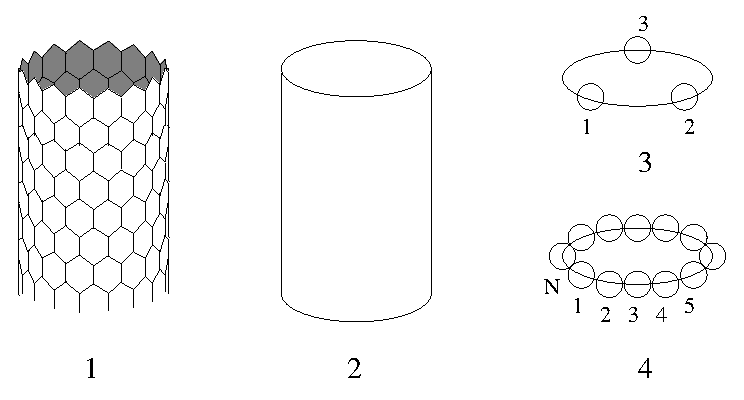
\includegraphics[clip]{1995phy5-1.eps}}
\end{center}

\end{question}
\begin{answer}{専攻 問題5}{}

\begin{subanswers}
\SubAnswer
  \begin{subsubanswers}
  \SubSubAnswer
    自由電子のSchr\"{o}dinger方程式は
%
    \[ -\frac{\hbar^2}{2m} \Laplacian \psi= E\psi \]
%
    円筒座標系で考える。ラプラシアンは
%
    \[ \Laplacian = \Partial{^2}{r^2} + \frac{1}{r}\Partial{}{r}%
                  + \frac{1}{r^2}\Partial{^2}{\theta^2}%
                  + \Partial{^2}{z^2} \]
%
    であるが、電子は円筒面上のみ動くので動径方向の偏微分は作用して
    も消えてしまう。よって
%
    \[ -\frac{\hbar^2}{2m} \Laplacian \psi(\theta,z)%
       = -\frac{\hbar^2}{2m} \left(%
           \frac{1}{r^2}\Partial{^2}{\theta^2}+\Partial{^2}{z^2}%
         \right) \psi(\theta,z) = E \psi(\theta,z) \]
%
    となる。$\psi(\theta,z)=\Theta(\theta)Z(z)$ と変数分離する。
%
    \[ -\frac{\hbar^2}{2mr^2} \Partial{^2\Theta}{\theta^2}%
        = E_\theta\Theta \hspace{15mm}%
       -\frac{\hbar^2}{2m}\Partial{^2Z}{z^2}%
        = E_z Z \hspace{15mm}%
        ( E = E_\theta+E_z ) \]
%
    従って、上式を満たす固有関数は
%
    \[ \Theta(\theta) = e^{ik_\theta r\theta} \hspace{10mm}%
       Z(z)           = e^{ik_zz} \hspace{10mm}%
       (k_\theta=\frac{\sqrt{2mE_\theta}}{\hbar} \quad%
        k_z=\frac{\sqrt{2mE_z}}{\hbar}) \]
%
    周期的境界条件 $\Theta(\theta+2\pi)=\Theta(\theta)$、$Z(z+L)=Z(z)$
    より
%
    \[ k_\theta=\frac{n_\theta}{r} \hspace{10mm}%
       k_z     =\frac{2\pi n_z}{L} \hspace{10mm}%
       (n_\theta,n_z=0,\pm 1,\pm 2,\cdots) \]
%
    以上より固有関数 $\psi(\theta,z)$ と固有エネルギー $E$ は
%
    \[ \psi(\theta,z) = \Theta(\theta)Z(z)%
                      = e^{i(n_\theta\theta+\frac{2\pi n_z}{L}z)} \]
    \[ E = E_\theta+E_z%
         = \frac{\hbar^2}{2m} \left\{%
             \left(\frac{n_\theta}{r}\right)^2%
            +\left(\frac{2\pi n_z}{L}\right)^2%
           \right\} \hspace{15mm}%
           (n_\theta,n_z=0,\pm 1,\pm 2,\cdots) \]
%
    である。


  \SubSubAnswer
    長さ $L$ の周期的境界条件をもつ1次元の系の波動関数として$Z(z)$
    が前問で得られている。それによると $k_z$の波数空間は $2\pi/L$ で
    離散化している。またエネルギー $E_z$ に対応する波数は
%
    \[ k_z = \pm\frac{\sqrt{2mE_z}}{\hbar} \]
%
    であるので、エネルギーが $E_z$ 以下である状態の数 $N(E_z)$ は
%
    \[ N(E_z) = 2 \cdot \frac{L}{2\pi} \frac{\sqrt{2mE_z}}{\hbar}%
              = \frac{L\sqrt{2mE_z}}{\pi\hbar} \]
%
    となる。下図参照。
%
    \begin{center}
      \mbox{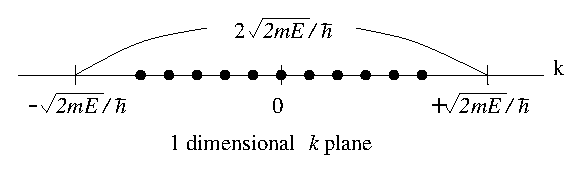
\includegraphics[clip]{1995phy5-2.eps}}
    \end{center}
%
    よって1次元の状態密度 $D^{(1)}(E_z)$ は
%
    \[ D^{(1)}(E_z) = \Deriver{N(E_z)}{E_z}%
      = \frac{L}{\pi\hbar}\sqrt{\frac{m}{2}} \frac{1}{\sqrt{E_z}} \]
%
    これをもとに、円筒上の2次元$k$空間における状態の数を数える。
    $k_z=\frac{2\pi}{L}n_z,\,k_\theta=\frac{n_\theta}{r}$
    が張る平面を考えると、$L$ は $r$に比べ十分に大きいから、
    次の図のように $k_z$ 方向にほぼ連続で、$k_\theta$ 方向には
    離散化した平面になっている。各$k_\theta$で、 $k_z$ に関する
    状態密度 $D^{(1)}(E_z)$ を足し上げたものが
    求める2次元状態密度 $D^{(2)}(E)$ になっている。
%
    \begin{center}\vspace*{-2mm}
      \mbox{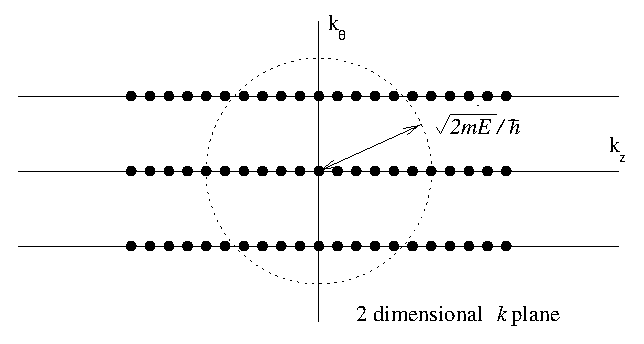
\includegraphics[clip]{1995phy5-3.eps}}
    \end{center}
%
    半径 $\frac{\sqrt{2mE}}{\hbar}$ の円を考えると、
    $k_\theta=\frac{n_{\theta}}{r}$
    での状態密度 $D^{(1)}_{n_{\theta}}(E)$ は
%
    \[ D^{(1)}_{n_{\theta}}(E)%
        = D^{(1)}\left(E-\frac{\hbar^2n_{\theta}^2}{2mr^2}\right)%
        = \frac{L}{\pi\hbar}\sqrt{\frac{m}{2}} \left(%
            E-\frac{\hbar^2n_{\theta}^2}{2mr^2}
          \right)^{-\frac{1}{2}} \]
%
    従って、求める状態密度 $D^{(2)}(E)$ は、($k_\theta$方向に十分
    密でないので、積分公式が使えないことに注意。)
%
    \begin{eqnarray*}
      D^{(2)}(E) &=&  D^{(1)}_{n_{\theta}=0}(E)%
                  + 2\sum_{n_{\theta}=1}^{n_{\theta_{\rm max}}}%
                    D^{(1)}_{n_{\theta}}(E) \\
               &=&  \frac{L}{\pi\hbar}\sqrt{\frac{m}{2}}%
                    \left\{%
                       E^{-\frac{1}{2}}%
                     + 2\sum_{n=1}^{n_{\theta_{\rm max}}} \left(%
                          E-\frac{\hbar^2n_{\theta}^2}{2mr^2}%
                       \right)^{-\frac{1}{2}}%
                    \right\}
    \end{eqnarray*}
%
    ただし、$n_{\theta_{\rm max}}$ は
    $\frac{\hbar^2n_{\theta_{\rm max}}^2}{2mr^2}\leq E$
    を満たす最大の整数である。\\
%
    $L\gg r$ のとき、状態密度の概形は次の図のとおりである。
    $E=\frac{\hbar^2n^2}{2mr^2}$ ごとに大きなとびが現れる。
%
    \begin{center}
      \mbox{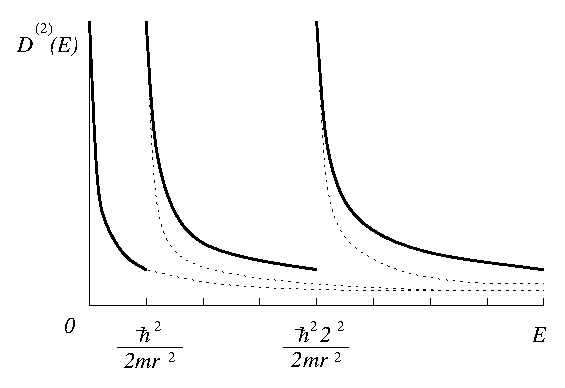
\includegraphics[clip]{1995phy5-4.eps}}\\
      状態密度の概形。
    \end{center}

  \end{subsubanswers}

\SubAnswer
  \begin{subsubanswers}
  \SubSubAnswer
    \parbox[t]{95mm}{
    与えられたハミルトニハン${\cal H}$ の行列表現の固有値 $E$を
    求めれば良い。
%
    \[ \left|\begin{matrix}%
          \eps-E & t & t \\
          t & \eps-E & t \\
          t & t & \eps-E
       \end{matrix}\right|%
       = (\eps-E+2t)(\eps-E-t)^2  \]
%
    よって固有値 $E$ は
%
    \[ E = \eps+2t\,(1重),\quad \eps-t\,(2重) \]
%
    となり、エネルギーの縮退が解ける。この様子を右図に示す。
%
    }\parbox[t]{55mm}{
    \begin{center}
       \mbox{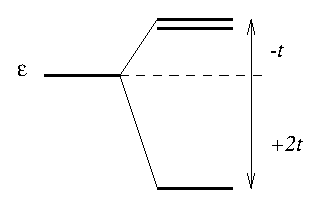
\includegraphics[clip]{1995phy5-5.eps}}
    \end{center}}
%


  \SubSubAnswer
    輪を回る電子の固有波動関数が各原子に局在した電子の固有波動関数
    の線形結合で記述できるとする。すなわち、
%
    \[ \psi = \sum_{n=1}^N c_n \phi_n \]
%
    このとき、
%
    {
    \def\e{\eps}
    \def\d{\ddots}
%
    \begin{eqnarray}
	 \begin{pmatrix}%
         \e & t  & 0  &    & 0  & t  \\
         t  & \e & \d & \d &    & 0  \\
         0  & \d & \d & \d & \d &    \\
            & \d & \d & \d & \d & 0  \\
         0  &    & \d & \d & \e & t  \\
         t  & 0  &    & 0  & t  & \e
       \end{pmatrix}%
       \begin{pmatrix}%
         c_1 \cr c_2 \\ \vdots \\ \vdots \\ c_{N-1} \\ c_N
       \end{pmatrix}%
       = E%
       \begin{pmatrix}%
         c_1 \\ c_2 \\ \vdots \\ \vdots \\ c_{N-1} \\ c_N
       \end{pmatrix}%
	\eqname{mateq}
    \end{eqnarray}
    }
%
    をみたす$c_n$および、$E$をもとめればよい。
    そこで、
\[
	c_n = c e^{inka}\hspace{10mm} (n=1,2,\cdots,N)
\]
    を仮定してみる。すると、この連立方程式の任意の式は
    \[ 
	t c_{n-1} + \eps c_{n} + t c_{n+1} = E c_{n} 
        \qquad \Yueni E = \eps + 2t \cos{ka} 
    \]

    従って、この$E$および、$c_n$の組は確かに\eqhref{mateq}の解になっ
    ている。

    次に、$k$のとり得る値であるが、$c_{N+1}=c_1$ の周期条件があるため
\[
  k = \frac{2\pi}{aN}\ell \hspace{10mm}%
       (\ell=0,1,\cdots,N-1) 
\]
となる。したがって、\eqhref{mateq}をみたす$N$個の固有値
\[
   E = \eps + 2t \cos{ka} \qquad k = \frac{2\pi}{aN}\ell \hspace{10mm}%
       (\ell=0,1,\cdots,N-1) 
\]
が得られた。

  \SubSubAnswer
    前問の結果より、大きい$N$には小さな $k$ が存在する。
    $ka\ll 1$ では、
%
    \[ E = \eps+2t\cos(ka)%
    \simeq \eps+2t\left(1-\frac{(ka)^2}{2}\right)%
         = \eps+2t-ta^2k^2 \]
%
    と近似できるが、$-ta^2>0$ より、エネルギーの $k$ 依存性は、
    定数項 $\eps+2t$ を別として、自由電子
    $E=\frac{\hbar^2}{2m^{*}}k^2$ の様に振舞う。すなわち、
%
    \[ -ta^2 = \frac{\hbar^2}{2m^{*}} \hspace{10mm}%
         \Yueni m^{*} = -\frac{\hbar^2}{2ta^2} \]
%
    質量$m^{*}$がこのように与えられる自由電子と見ることができる。

  \end{subsubanswers}
\end{subanswers}
\end{answer}


\end{document}
